	%%%%%%%%%%%%%%%%%%%%%%%%%%%%%%%%%%%%%%%%%%%%%%%%%%%%%%%%%%%%%%%%
%
%  Template for homework of Introduction to Machine Learning.
%
%  Fill in your name, lecture number, lecture date and body
%  of homework as indicated below.
%
%%%%%%%%%%%%%%%%%%%%%%%%%%%%%%%%%%%%%%%%%%%%%%%%%%%%%%%%%%%%%%%%
\documentclass[11pt,letter,notitlepage]{article}
%Mise en page
\usepackage[left=2cm, right=2cm, lines=45, top=0.8in, bottom=0.7in]{geometry}
\usepackage{fancyhdr}
\usepackage{fancybox}
\usepackage{graphicx}
\usepackage{pdfpages}
\usepackage{enumitem}
\usepackage{algorithm}
\usepackage{algorithmic}
\renewcommand{\headrulewidth}{1.5pt}
\renewcommand{\footrulewidth}{1.5pt}
\newcommand\Loadedframemethod{TikZ}
\renewcommand{\thefootnote}{}

\usepackage[framemethod=\Loadedframemethod]{mdframed}
\usepackage{amssymb,amsmath,bm}
\usepackage{amsthm}
\usepackage{thmtools}
\usepackage{extarrows}
\usepackage{mathtools}
\usepackage{pifont}
\setlength{\topmargin}{0pt}
\setlength{\textheight}{9in}
\setlength{\headheight}{0pt}
\setlength{\oddsidemargin}{0.25in}
\setlength{\textwidth}{6in}
%%%%%%%%%%%%%%%%%%%%%%%%
%%%%%% Define math operator %%%%%
%%%%%%%%%%%%%%%%%%%%%%%%
\DeclareMathOperator*{\argmin}{\bf argmin}
\DeclareMathOperator*{\relint}{\bf relint\,}
\DeclareMathOperator*{\dom}{\bf dom\,}
\DeclareMathOperator*{\intp}{\bf int\,}
%%%%%%%%%%%%%%%%%%%%%%%
\setlength{\topmargin}{0pt}
\setlength{\textheight}{9in}
\setlength{\headheight}{0pt}
\setlength{\oddsidemargin}{0.25in}
\setlength{\textwidth}{6in}
\pagestyle{fancy}
%%%%%%%%%%%%%%%%%%%%%%%%
%% Define the Exercise environment %%
%%%%%%%%%%%%%%%%%%%%%%%%
\mdtheorem[
topline=false,
rightline=false,
leftline=false,
bottomline=false,
leftmargin=-10,
rightmargin=-10
]{exercise}{\textbf{Exercise}}
%%%%%%%%%%%%%%%%%%%%%%%
%% End of the Exercise environment %%
%%%%%%%%%%%%%%%%%%%%%%%
%%%%%%%%%%%%%%%%%%%%%%%%
%% Define the Problem environment %%
%%%%%%%%%%%%%%%%%%%%%%%%
\mdtheorem[
topline=false,
rightline=false,
leftline=false,
bottomline=false,
leftmargin=-10,
rightmargin=-10
]{problem}{\textbf{Problem}}
%%%%%%%%%%%%%%%%%%%%%%%
%% End of the Exercise environment %%
%%%%%%%%%%%%%%%%%%%%%%%
%%%%%%%%%%%%%%%%%%%%%%%
%% Define the Solution Environment %%
%%%%%%%%%%%%%%%%%%%%%%%
\declaretheoremstyle
[
spaceabove=0pt,
spacebelow=0pt,
headfont=\normalfont\bfseries,
notefont=\mdseries,
notebraces={(}{)},
headpunct={:\;},
headindent={},
postheadspace={ },
bodyfont=\normalfont,
qed=$\blacksquare$,
preheadhook={\begin{mdframed}[style=myframedstyle]},
postfoothook=\end{mdframed},
]{mystyle}
\declaretheorem[style=mystyle,title=Solution]{solution}
\mdfdefinestyle{myframedstyle}{%
	topline=false,
	rightline=false,
	leftline=false,
	bottomline=false,
	skipabove=-6ex,
	leftmargin=-10,
	rightmargin=-10,
	backgroundcolor=black!5}
%%%%%%%%%%%%%%%%%%%%%%%
%% End of the Solution environment %%
%%%%%%%%%%%%%%%%%%%%%%%

%% Homework info.
\newcommand{\posted}{\text{Oct. 15, 2024}}       			%%% FILL IN POST DATE HERE
\newcommand{\due}{\text{Oct. 24, 2024}} 			%%% FILL IN Due DATE HERE
\newcommand{\hwno}{\text{2}} 		           			%%% FILL IN LECTURE NUMBER HERE


%%%%%%%%%%%%%%%%%%%%
%% Put your information here %%
%%%%%%%%%%%%%%%%%%%
\newcommand{\name}{\text{San Zhang}}  	          			%%% FILL IN YOUR NAME HERE
\newcommand{\id}{\text{PBXXXXXXXX}}		       			%%% FILL IN YOUR ID HERE
%%%%%%%%%%%%%%%%%%%%
%% End of the student's info %%
%%%%%%%%%%%%%%%%%%%


\newcommand{\proj}[2]{\textbf{P}_{#2} (#1)}
\newcommand{\lspan}[1]{\textbf{span}  (#1)  }
\newcommand{\rank}[1]{ \textbf{rank}  (#1)  }
\newcommand{\RNum}[1]{\uppercase\expandafter{\romannumeral #1\relax}}
\DeclareMathOperator*{\cl}{\bf cl\,}
\DeclareMathOperator*{\bd}{\bf bd\,}
\DeclareMathOperator*{\conv}{\bf conv\,}
\DeclareMathOperator*{\epi}{\bf epi\,}


% \lhead{
% 	\textbf{\name}
% }
% \rhead{
% 	\textbf{\id}
% }
\chead{\textbf{Homework\hwno}}


\begin{document}
\vspace*{-4\baselineskip}
\thispagestyle{empty}


\begin{center}
{\bf\large Introduction to Machine Learning}\\
{Fall 2024}\\
University of Science and Technology of China
\end{center}

\noindent
Lecturer: Jie Wang  			 %%% FILL IN LECTURER HERE
\hfill
Homework \hwno             			
\\
Posted: \posted
\hfill
Due: \due
%\\
% Name: \name             			
% \hfill
% ID: \id						
% \hfill

\noindent
\rule{\textwidth}{2pt}

\medskip





%%%%%%%%%%%%%%%%%%%%%%%%%%%%%%%%%%%%%%%%%%%%%%%%%%%%%%%%%%%%%%%%
%% BODY OF HOMEWORK GOES HERE
%%%%%%%%%%%%%%%%%%%%%%%%%%%%%%%%%%%%%%%%%%%%%%%%%%%%%%%%%%%%%%%%

\textbf{Notice, }to get the full credits, please present your solutions step by step.
	
	\begin{exercise}[Projection ]
		Let $\mathbf{A}\in\mathbb{R}^{m\times n}$ and $\mathbf{x} \in \mathbb{R}^m$. Define
		\begin{align*}
			\proj{\mathbf{x}}{\mathbf{A}} = \argmin_{\mathbf{z}\in\mathbb{R}^m}\,\{\|\mathbf{x}-\mathbf{z}\|_2: \mathbf{z}\in\mathcal{C}(\mathbf{A})\}.
		\end{align*}
		We call $\proj{\mathbf{x}}{\mathbf{A}}$ the projection of the point $\mathbf{x}$ onto the column space of $\mathbf{A}$.
		\begin{enumerate}
			\item Please prove that $\mathbf{P}_{\mathbf{A}}(\mathbf{x})$ is unique for any $\mathbf{x} \in \mathbb{R}^m$.
			\item Let $\mathbf{v}_i \in \mathbb{R}^n$, $i=1,\ldots,d$ with $d\leq n$, which are linearly independent.
			\begin{enumerate}
				\item For any $\mathbf{w}\in \mathbb{R}^n$, please find $\proj{\mathbf{w}}{\mathbf{v}_1}$, which is the projection of $\mathbf{w}$ onto the subspace spanned by $\mathbf{v}_1$.
				\item Please show $\proj{\cdot}{\mathbf{v}_1}$ is a linear map, i.e.,
				\begin{align*}
					\proj{\alpha\mathbf{u}+\beta\mathbf{w}}{\mathbf{v}_1}=\alpha\proj{\mathbf{u}}{\mathbf{v}_1} + \beta \proj{\mathbf{w}}{\mathbf{v}_1},
				\end{align*}
				where $\alpha,\beta\in\mathbb{R}$ and $\mathbf{w}\in\mathbb{R}^n$.
				\item Please find the projection matrix corresponding to the linear map $\proj{\cdot}{\mathbf{v}_1}$, i.e., find the matrix $\mathbf{H}_1\in\mathbb{R}^{n\times n}$ such that
				\begin{align*}
					\proj{\mathbf{w}}{\mathbf{v}_1}=\mathbf{H}_1\mathbf{w}.
				\end{align*}
				\item Let $\mathbf{V}=(\mathbf{v}_1,\ldots,\mathbf{v}_d)$, and $\mathbf{v}_1,\ldots,\mathbf{v}_d$ are linearly independent.
                % added by haotonghuang
				\begin{enumerate}
					\item For any $\mathbf{w}\in \mathbb{R}^n$, please find $\proj{\mathbf{w}}{\mathbf{V}}$ and the corresponding projection matrix $\mathbf{H}$.
					\item Please find $\mathbf{H}$ if we further assume that $\mathbf{v}_i^{\top}\mathbf{v}_j=0$, $\forall\,i\neq j$.
				\end{enumerate}
			\end{enumerate}
			
			\item
			\begin{enumerate}
				\item Suppose that
				\begin{align*}
					\mathbf{A} = \left[
					\begin{matrix}
						1 & 0\\
						0 & 1
					\end{matrix}
					\right] .
				\end{align*}
				What are the coordinates of $\mathbf{P}_{\mathbf{A}}(\mathbf{x})$ with respect to the column vectors in $\mathbf{A}$ for any $\mathbf{x} \in \mathbb{R}^2$? Are the coordinates unique?
				\item Suppose that
				\begin{align*}
					\mathbf{A} = \left[
					\begin{matrix}
						1 & 2\\
						1 & 2
					\end{matrix}
					\right] .
				\end{align*}
				What are the coordinates of $\mathbf{P}_{\mathbf{A}}(\mathbf{x})$ with respect to the column vectors in $\mathbf{A}$ for any $\mathbf{x} \in \mathbb{R}^2$? Are the coordinates unique?
			\end{enumerate}
			
			\item (Optional) A matrix $\mathbf{P}$ is called a projection matrix if $\mathbf{P}\mathbf{x}$ is the projection of $\mathbf{x}$ onto $\mathcal{C}(\mathbf{P})$ for any $\mathbf{x}$.
			\begin{enumerate}
				\item Let $\lambda$ be the eigenvalue of $\mathbf{P}$. Show that $\lambda$ is either $1$ or $0$. (\emph{Hint: you may want to figure out what the eigenspaces corresponding to $\lambda=1$ and $\lambda=0$ are, respectively.})
				\item Show that $\mathbf{P}$ is a projection matrix if and only if $\mathbf{P}^2 = \mathbf{P}$ and $\mathbf{P}$ is symmetric.
			\end{enumerate}
			
			\item (Optional) Let $\mathbf{B} \in \mathbb{R}^{m\times s}$ and $\mathcal{C}(\mathbf{B}) $ be its column space. Suppose that $\mathcal{C}(\mathbf{B})$ is a proper subspace of $ \mathcal{C}(\mathbf{A})$.
			Is $\proj{\mathbf{x}}{\mathbf{B}}$ the same as $\proj{\proj{\mathbf{x}}{\mathbf{A}}}{\mathbf{B}}$? Please show your claim rigorously.
		\end{enumerate}
	\end{exercise}

\newpage

\begin{solution}\textbf{Projection}
\begin{enumerate}
	\item
	\ding{172} Strict Convexity:

	Define
	$$f(\mathbf{z}) = \Vert \mathbf{x} - \mathbf{z} \Vert_2^2 = \Vert \mathbf{z} \Vert_2^2 + 2\langle \mathbf{x}, \mathbf{z} \rangle + \Vert \mathbf{x} \Vert_2^2$$
	Then $\nabla^2 f(\mathbf{z}) = 2 \mathbf{I_m} > 0$ $\Longrightarrow$ $f$ is strictly convex. 
	
	The column space $\mathcal{C}(\mathbf{A})$ is convex $\Longrightarrow$ $\forall$ $\mathbf{a}, \mathbf{b} \in \mathcal{C}(\mathbf{A})$, $\forall$ $t \in (0,1)$, $t\mathbf{a} + (1-t)\mathbf{b} \in \mathcal{C}(\mathbf{A})$. 
	
	Suppose $\mathbf{z_1}, \mathbf{z_2} \in \mathcal{C}(\mathbf{A})$ are both minimizers of $f$ over $\mathcal{C}(\mathbf{A})$. Then according to the convexity of $f$,
	\[
	f(t\mathbf{z_1} + (1-t)\mathbf{z_2}) < tf(\mathbf{z_1}) + (1-t)f(\mathbf{z_2}) = f(\mathbf{z_1}) = f(\mathbf{z_2})
	\]
	contradicting the minimality of $\mathbf{z_1}$ and $\mathbf{z_2}$. Therefore, the minimizer $\proj{\mathbf{x}}{\mathbf{A}}$ is unique.

	\ding{173} Orthogonality:
	
	Suppose $\mathbf{z_0}$ is a minimizer of $f$ over $\mathcal{C}(\mathbf{A})$. For any $\mathbf{y} \in \mathcal{C}(\mathbf{A})$ and $t \in \mathbb{R}$, define
	$$\Phi(t) = \Vert \mathbf{x}-(\mathbf{z_0} + t\mathbf{y}) \Vert_2^2 = \Vert \mathbf{x} - \mathbf{z_0} \Vert_2^2 - 2t\langle\mathbf{x}-\mathbf{z_0}, \mathbf{y}\rangle + t^2 \Vert \mathbf{y} \Vert_2^2$$
	Notice that $\mathbf{z_0} + t\mathbf{y} \in \mathcal{C}(\mathbf{A})$.

	Since $\mathbf{z_0}$ minimizes $f$ over $\mathcal{C}(\mathbf{A})$, $\Phi(t)$ achieves its minimum at $t = 0$ $\Longrightarrow$ $\Phi'(0) = -2 \langle \mathbf{x} - \mathbf{z_0}, \mathbf{y} \rangle = 0$ $\Longrightarrow$ $\mathbf{x} - \mathbf{z_0} \perp \mathcal{C}(\mathbf{A})$, i.e., $\mathbf{x} - \mathbf{z_0} \in \mathcal{C}(\mathbf{A})^{\perp}$.

	Fruthermore, if $\mathbf{x} - \mathbf{z_0} \perp \mathcal{C}(\mathbf{A})$, then for any $\mathbf{y} \in \mathcal{C}(\mathbf{A})$,
	\[
	\Vert \mathbf{x} - \mathbf{y} \Vert_2^2 = \Vert \mathbf{x} - \mathbf{z_0} + \mathbf{z_0} - \mathbf{y} \Vert_2^2 = \Vert \mathbf{x} - \mathbf{z_0} \Vert_2^2 + \Vert \mathbf{z_0} - \mathbf{y} \Vert_2^2 \geq \Vert \mathbf{x} - \mathbf{z_0} \Vert_2^2
	\]
	$\Longrightarrow$ $\mathbf{z_0}$ is a minimizer of $f$ over $\mathcal{C}(\mathbf{A})$.

	If $\mathbf{z_1}$, $\mathbf{z_2}$ both satisfy $\mathbf{x} - \mathbf{z_i} \perp \mathcal{C}(\mathbf{A})$ ($i = 1,2$), then $\mathbf{z_1} - \mathbf{z_2} \in \mathcal{C}(\mathbf{A})$ and $\mathbf{z_1} - \mathbf{z_2} = (\mathbf{x} - \mathbf{z_2}) - (\mathbf{x} - \mathbf{z_1}) \perp \mathcal{C}(\mathbf{A})$ $\Longrightarrow$ $\mathbf{z_1} - \mathbf{z_2} = \mathbf{0}$ $\Longrightarrow$ $\mathbf{z_1} = \mathbf{z_2}$, i.e. the minimizer $\proj{\mathbf{x}}{\mathbf{A}}$ is unique.
	\item 
	\begin{enumerate}
		\item 
		\[
		\proj{\mathbf{w}}{\mathbf{v}_1}
		=
		\argmin_{\substack{\alpha \mathbf{v_1} \\ \alpha \in \mathbb{R}, \mathbf{v}_1 \in \mathbb{R}^n}} \Vert \mathbf{w} - \alpha \mathbf{v}_1 \Vert_2
		\]
		\[
		\frac{\mathrm{d}}{\mathrm{d} \alpha} \Vert \mathbf{w} - \alpha \mathbf{v}_1 \Vert_2^2
		=
		\frac{\mathrm{d}}{\mathrm{d} \alpha} (\mathbf{w} - \alpha \mathbf{v}_1)^{\top}(\mathbf{w} - \alpha \mathbf{v}_1)
		=
		-2\mathbf{v}_1^{\top}(\mathbf{w} - \alpha \mathbf{v}_1)
		=
		0
		\]
		\[
		\Longrightarrow
		\alpha^*
		=
		\frac{\mathbf{v_1^T}\mathbf{w}}{\mathbf{v_1^T}\mathbf{v_1}}
		\Longrightarrow
		\proj{\mathbf{w}}{\mathbf{v}_1}
		=
		\frac{\mathbf{v_1^T}\mathbf{w}}{\mathbf{v_1^T}\mathbf{v_1}}\mathbf{v}_1
		\]
		\item 
		According to the result in (a),
		\begin{align*}
		\proj{\alpha \mathbf{u} + \beta \mathbf{w}}{\mathbf{v}_1}
		=
		\frac{\mathbf{v_1^T}(\alpha \mathbf{u} + \beta \mathbf{w})}{\mathbf{v_1^T}\mathbf{v_1}}\mathbf{v}_1
		&=
		\alpha \frac{\mathbf{v_1^T}\mathbf{u}}{\mathbf{v_1^T}\mathbf{v_1}}\mathbf{v}_1
		+
		\beta \frac{\mathbf{v_1^T}\mathbf{w}}{\mathbf{v_1^T}\mathbf{v_1}}\mathbf{v}_1\\
		&=
		\alpha \proj{\mathbf{u}}{\mathbf{v}_1} + \beta \proj{\mathbf{w}}{\mathbf{v}_1}
		\end{align*}
		\item 
		\[
		\proj{\mathbf{w}}{\mathbf{v}_1}
		=
		\frac{\mathbf{v_1^T}\mathbf{w}}{\mathbf{v_1^T}\mathbf{v_1}}\mathbf{v}_1
		=
		\left(\frac{\mathbf{v_1}\mathbf{v_1^T}}{\mathbf{v_1^T}\mathbf{v_1}}\right)\mathbf{w}
		:=
		\mathbf{H_1} \mathbf{w}
		\]
		\item 
		\begin{enumerate}
			\item 
			\[\proj{\mathbf{w}}{\mathbf{V}}
			=
			\argmin_{\substack{\mathbf{Vy} \\ \mathbf{y} \in \mathbb{R}^d, \mathbf{V} \in \mathbb{R}^{n \times d}}} \Vert \mathbf{w} - \mathbf{Vy} \Vert_2
			\]
			\[
			\frac{\mathrm{d}}{\mathrm{d} \mathbf{y}} \Vert \mathbf{w} - \mathbf{Vy} \Vert_2^2
			=
			\frac{\mathrm{d}}{\mathrm{d} \mathbf{y}} (\mathbf{w} - \mathbf{Vy})^{\top}(\mathbf{w} - \mathbf{Vy})
			=
			-2\mathbf{V}^{\top}(\mathbf{w} - \mathbf{Vy})
			=
			0
			\]
			$\mathbf{v_i}$, $i=1,\ldots,d$ are linearly independent $\Longrightarrow$ $\mathbf{V}$ has full column rank $\Longrightarrow$ $\mathbf{V}^{\top}\mathbf{V}$ is invertible.
			\[
			\Longrightarrow
			\mathbf{y}^*
			=
			(\mathbf{V}^{\top}\mathbf{V})^{-1}\mathbf{V}^{\top}\mathbf{w}
			\Longrightarrow
			\proj{\mathbf{w}}{\mathbf{V}}
			=
			\mathbf{V}(\mathbf{V}^{\top}\mathbf{V})^{-1}\mathbf{V}^{\top}\mathbf{w}
			\]
			\[
			\Longrightarrow
			\mathbf{H}
			=
			\mathbf{V}(\mathbf{V}^{\top}\mathbf{V})^{-1}\mathbf{V}^{\top}
			\]
			\item 
			\begin{align*}
			\mathbf{v_i^T}\mathbf{v_j}
			=
			0, \forall i \neq j
			&\Longrightarrow
			\mathbf{V}^{\top}\mathbf{V}
			=
			\left[\begin{matrix}
			\mathbf{v_1^T}\mathbf{v_1} & 0 & \cdots & 0\\
			0 & \mathbf{v_2^T}\mathbf{v_2} & \cdots & 0\\
			\vdots & \vdots & \ddots & \vdots\\
			0 & 0 & \cdots & \mathbf{v_d^T}\mathbf{v_d}
			\end{matrix}\right]\\
			&\Longrightarrow
			(\mathbf{V}^{\top}\mathbf{V})^{-1}
			=
			\left[\begin{matrix}
			\frac{1}{\mathbf{v_1^T}\mathbf{v_1}} & 0 & \cdots & 0\\
			0 & \frac{1}{\mathbf{v_2^T}\mathbf{v_2}} & \cdots & 0\\
			\vdots & \vdots & \ddots & \vdots\\
			0 & 0 & \cdots & \frac{1}{\mathbf{v_d^T}\mathbf{v_d}}
			\end{matrix}\right]\\
			&\Longrightarrow
			\mathbf{H}
			=
			\sum\limits_{i=1}^{d} \frac{\mathbf{v_i}\mathbf{v_i^T}}{\mathbf{v_i^T}\mathbf{v_i}}
			\end{align*}
		\end{enumerate}
	\end{enumerate}
	\item 
	\begin{enumerate}
		\item 
		\[
		\mathbf{A} = \left[
		\begin{matrix}
			1 & 0\\
			0 & 1
		\end{matrix}
		\right]
		\Longrightarrow
		\mathbf{x}
		\in
		\mathcal{C}(\mathbf{A}) = \mathbb{R}^2
		\Longrightarrow
		\proj{\mathbf{x}}{\mathbf{A}} 
		= 
		\mathbf{x}
		=
		\mathbf{A}
		\cdot
		\mathbf{x}
		\]
		The coordinates of $\mathbf{P_A}(\mathbf{x})$ with respect to the column vectors in $\mathbf{A}$ are unique and equal to $\mathbf{x}$ itself.
		\item
		\[
		\mathbf{A} = \left[
		\begin{matrix}
			1 & 2\\
			1 & 2
		\end{matrix}
		\right]
		\Longrightarrow
		\mathcal{C}(\mathbf{A}) = \{\alpha (1,1)^T : \alpha \in \mathbb{R}\}
		\]
		\[
		\proj{\mathbf{x}}{\mathbf{A}}
		=
		\argmin_{\substack{\alpha (1,1)^T \\ \alpha \in \mathbb{R}}} \Vert \mathbf{x} - \alpha (1,1)^T \Vert_2
		\]
		\[
		\xrightarrow{2.(a)}
		\proj{\mathbf{x}}{\mathbf{A}}
		=
		\frac{(1,1)\mathbf{x}}{(1,1)(1,1)^T}(1,1)^T
		=
		\frac{x_1 + x_2}{2}(1,1)^T
		=
		\mathbf{A}
		\cdot
		\left(c_1, c_2\right)^T
		\]
		$\Longrightarrow$ The set of all coordinates of $\mathbf{P_A}(\mathbf{x})$ with respect to the column vectors in $\mathbf{A}$ is the affine line:
		\[
		\left\{(c_1, c_2)^T \in \mathbb{R}^2 : c_1 + 2c_2 = \frac{x_1 + x_2}{2}\right\}
		\]
		Thus the coordinates are not unique.	
	\end{enumerate}
	\item 
	\begin{enumerate}
		\item 
		Let $\lambda$ be an eigenvalue of $\mathbf{P}$ and $\mathbf{v}$ be the corresponding eigenvector. Then $\mathbf{P}\mathbf{v} = \lambda \mathbf{v}$. Since $\mathbf{P}$ is a projection matrix, $\mathbf{P}\mathbf{v}$ is the projection of $\mathbf{v}$ onto $\mathcal{C}(\mathbf{P})$ $\Longrightarrow$ $\mathbf{v} = \mathbf{P}\mathbf{v} + \left(\mathbf{v} - \mathbf{P}\mathbf{v}\right)$, where $\mathbf{P}\mathbf{v} \in \mathcal{C}(\mathbf{P})$ and $\mathbf{v} - \mathbf{P}\mathbf{v} \in \mathcal{C}(\mathbf{P})^{\perp}$.
		\[
		\Longrightarrow
		\Vert \mathbf{v} \Vert_2^2
		=
		\Vert \mathbf{Pv} \Vert_2^2
		+
		\Vert \mathbf{v} - \mathbf{Pv} \Vert_2^2
		\xRightarrow{\mathbf{Pv} = \lambda \mathbf{v}}
		\left(\lambda^2-\lambda\right)\Vert \mathbf{v} \Vert_2^2
		=
		0
		\Longrightarrow
		\lambda \in \{0, 1\}
		\]
		\item
		\ding{172} Necessity:

		$\forall$ $\mathbf{x} \in \mathbb{R}^m$, $\mathbf{Px} \in \mathcal{C}(\mathbf{P})$. We need to prove that $\mathbf{x} - \mathbf{Px} \in \mathcal{C}(\mathbf{P})^{\perp}$.

		$\forall$ $\mathbf{y} \in \mathcal{C}(\mathbf{P})$, $\exists$ $\mathbf{z} \in \mathbb{R}^m$, s.t. $\mathbf{y} = \mathbf{Pz}$. Then
		\begin{align*}
		\langle \mathbf{x} - \mathbf{Px}, \mathbf{y} \rangle
		=
		\langle \mathbf{x} - \mathbf{Px}, \mathbf{Pz} \rangle
		&=
		\langle \mathbf{P^T}(\mathbf{x} - \mathbf{Px}), \mathbf{z} \rangle\\
		&\xlongequal{\mathbf{P^T} = \mathbf{P}}
		\langle \mathbf{P}(\mathbf{x} - \mathbf{Px}), \mathbf{z} \rangle\\
		&\xlongequal{\mathbf{P^2} = \mathbf{P}}
		\langle \mathbf{Px} - \mathbf{P}^2\mathbf{x}, \mathbf{z} \rangle
		=
		0
		\end{align*}
		$\Longrightarrow$ $\mathbf{x} - \mathbf{Px} \in \mathcal{C}(\mathbf{P})^{\perp}$ $\Longrightarrow$ $\mathbf{P}$ is a projection matrix.

		\ding{173} Sufficiency:

		$\mathbf{P}$ is a projection matrix $\Longrightarrow$ $\forall$ $\mathbf{x} \in \mathbb{R}^m$, $\mathbf{Px} \in \mathcal{C}(\mathbf{P})$
		
		$\Longrightarrow$ $\mathbf{P}(\mathbf{Px}) = \argmin_{\mathbf{z} \in \mathcal{C}(\mathbf{P})} \Vert \mathbf{Px} - \mathbf{z} \Vert_2 = \mathbf{Px}$ $\Longrightarrow$ $\mathbf{P^2} = \mathbf{P}$.

		$\mathbf{P}$ is a projection matrix $\Longrightarrow$ $\forall$ $\mathbf{x}, \mathbf{y} \in \mathbb{R}^m$, $\mathbf{x} = \mathbf{Px} + (\mathbf{x-Px})$, where $\mathbf{Px} \in \mathcal{C}(\mathbf{P})$ and $\mathbf{x-Px} \in \mathcal{C}(\mathbf{P})^{\perp}$. Since $\mathbf{Py} \in \mathcal{C}(\mathbf{P})$, we have
		\[
		\langle \mathbf{Px}, \mathbf{y} - \mathbf{Py} \rangle
		=
		0
		\Longrightarrow
		\langle \mathbf{Px}, \mathbf{y} \rangle
		=
		\langle \mathbf{Px}, \mathbf{Py} \rangle
		=
		\langle \mathbf{x}, \mathbf{Py} \rangle
		=
		\langle \mathbf{P^T x}, \mathbf{y} \rangle
		\]
		$\Longrightarrow$ $\mathbf{P^T} = \mathbf{P}$.
	\end{enumerate}
	\item $\forall$ $\mathbf{x} \in \mathbb{R}^m$,
	\[
	\mathcal{C}(\mathbf{B}) \text{ is a proper subspace of } \mathcal{C}(\mathbf{A})
	\Longrightarrow
	\forall \mathbf{z}\in\mathcal{C}(\mathbf{P}), z\in\mathcal{C}(\mathbf{A})
	\Longrightarrow
	\proj{\mathbf{x}}{\mathbf{A}} - \mathbf{z} \in \mathcal{C}(\mathbf{A})
	\]
	\begin{align*}
	\mathbf{x} - \proj{\mathbf{x}}{\mathbf{A}} \in \mathcal{C}(\mathbf{A})^{\perp}
	\Longrightarrow
	\Vert \mathbf{x} - z \Vert_2^2
	&=
	\Vert (\proj{\mathbf{x}}{\mathbf{A}} - \mathbf{z}) + \left(\mathbf{x}-\proj{\mathbf{x}}{\mathbf{A}}\right) \Vert_2^2\\
	&=
	\Vert \proj{\mathbf{x}}{\mathbf{A}} - \mathbf{z} \Vert_2^2
	+
	\Vert \mathbf{x}-\proj{\mathbf{x}}{\mathbf{A}} \Vert_2^2
	\end{align*}
	\[
	\Longrightarrow
	\argmin_{\mathbf{z} \in \mathcal{C}(\mathbf{B})} \Vert \mathbf{x} - \mathbf{z} \Vert_2
	=
	\argmin_{\mathbf{z} \in \mathcal{C}(\mathbf{B})} \Vert \proj{\mathbf{x}}{\mathbf{A}} - \mathbf{z} \Vert_2
	\Longrightarrow
	\proj{\mathbf{x}}{\mathbf{B}}
	=
	\proj{\proj{\mathbf{x}}{\mathbf{A}}}{\mathbf{B}}
	\]
\end{enumerate}
\end{solution}

\newpage
    \begin{exercise}[Projection to a Matrix Space]
        Let $\mathbb{R}^{n \times n}$ be the linear space of \(n \times n\) matrices. The inner product in this space is defined as \[ \langle A, B \rangle = \text{tr}(A^T B). \]
                \begin{enumerate}
                    \item Show that the set of diagonal matrices in $\mathbb{R}^{n \times n}$ forms a linear space. Besides, please find the the projection of any matrix onto the space of diagonal matrices.
                
                    \item Prove that the set of symmetric matrices, denoted $S^n$, in $\mathbb{R}^{n \times n}$ forms a linear space. Also, determine the dimension of this linear space.
    
                    \item Show that the inner product of any symmetric matrix and skew-symmetric matrix is zero. Moreover, prove that any matrix can be decomposed as the sum of a symmetric matrix and a skew-symmetric matrix.
    
                    \item Find the projection of any matrix onto the space of symmetric matrices.
                \end{enumerate}
    \end{exercise}
	
\newpage

\begin{solution} \textbf{Projection to a Matrix Space}
\begin{enumerate}
    \item
	Set $\mathcal{D} = \{D \in \mathbb{R}^{n \times n} \mid D \text{ is diagonal}\}$ as the set of diagonal matrices. 
	
	$\forall$ $D_1$, $D_2\in \mathcal{D}$ and $\alpha$, $\beta\in \mathbb{R}$, we have $\alpha D_1 + \beta D_2$ is diagonal $\Longrightarrow$ $\alpha D_1 + \beta D_2 \in \mathcal{D}$. Besides, $\mathbf{0} \in \mathcal{D}$.

	Hence $\mathcal{D}$ is a linear space.

	$\forall$ $A = (a_{ij})_{n\times n} \in \mathbb{R}^{n \times n}$, the projection of $A$ onto $\mathcal{D}$ is given by:
	\begin{align*}
	\mathbf{P}_{\mathcal{D}}(A)
	&=
	\argmin_{D = \text{diag}(x_1, \cdots, x_n) \in \mathcal{D}} \|A - D\|_F
	=
	\argmin_{D = \text{diag}(x_1, \cdots, x_n) \in \mathcal{D}} \|A - D\|_F^2\\
	&=
	\argmin_{D = \text{diag}(x_1, \cdots, x_n) \in \mathcal{D}} \langle A - D, A - D \rangle_F\\
	&=
	\argmin_{D = \text{diag}(x_1, \cdots, x_n) \in \mathcal{D}} \sum_{i,j} (a_{ij} - x_i \delta_{ij})^2
	=
	\argmin_{D = \text{diag}(x_1, \cdots, x_n) \in \mathcal{D}} \sum_{i} (a_{ii} - x_i)^2\\
	&=
	\text{diag}(a_{11}, \cdots, a_{nn})
	=
	\text{diag}(A)
	\end{align*}
	\item 
	$\forall$ $S_1$, $S_2\in S^n$ and $\alpha$, $\beta\in \mathbb{R}$, $(\alpha S_1 + \beta S_2)^\top = \alpha S_1^\top + \beta S_2^\top = \alpha S_1 + \beta S_2$ $\Longrightarrow$ $\alpha S_1 +\beta S_2 \in S^n$. Besides, $\mathbf{0} \in S^n$.

	Hence $S^n$ is a linear space.

	It is clear that there is a set of linearly independent basis that can represent all the matrices in the space:
	\[
	\{E_{ii}\}_{i=1}^{n} \cup \{E_{ij} + E_{ji}\}_{1 \leq i < j \leq n},
	\]
	where $E_{ij}$ is the matrix with $1$ in the $(i,j)$ position and $0$ elsewhere. 
	
	Therefore, 
	\[
	\dim S^n = n + \binom{n}{2} = \frac{n(n+1)}{2}.
	\]
	\item 
	Denote $K^n$ as the set of skew-symmetric matrices.
	
	Then $\forall$ $A \in S^n$ and $B \in K^n$, we have
	\begin{align*}
	\langle A, B \rangle
	=
	\text{tr}(A^\top B)
	&=
	\text{tr}(B^\top A)\\
	&\xlongequal{B \in K^n}
	-\text{tr}(BA)\\
	&\xlongequal{A \in S^n}
	-\text{tr}(B A^\top)
	=
	-\text{tr}(A^\top B)
	=
	-\langle A, B \rangle
	\Longrightarrow
	\langle A, B \rangle = 0.
	\end{align*}
	Decomposition:
	\[
	A \;=\; \underbrace{\frac{A + A^{\top}}{2}}_{\overset{\text{def}}{=}S(A)\in S^n}
	\;+\;
	\underbrace{\frac{A - A^{\top}}{2}}_{\overset{\text{def}}{=}K(A)\in K^n}.
	\]
	\item 
	According to (3), $A = S(A) + K(A)$, where $S(A) \in S^n$ and $K(A) \perp S^n$.

	Therefore, $\mathbf{P}_{S^n}(A) = S(A) = \frac{A + A^\top}{2}$.
\end{enumerate}
\end{solution}

\newpage
    \begin{exercise}[Projection to a Function Space]

        \begin{enumerate}
            % \item Let $\mathbf{X}\in \mathbb{R}^{n\times d}$ with rank $d$ and $\mathbf{y}\in \mathbb{R}^n$. Consider the optimization problem
            % \begin{align*}
            %     \min_{\mathbf{w}\in \mathbb{R}^d}\|\mathbf{y}-\mathbf{X w}\|_2^2,
            % \end{align*}
            % \begin{enumerate}
            %     \item  We denote the column space of $\mathbf{X}$ by $\mathcal{C}(\mathbf{X})$. Please show that $\hat{\mathbf{y}}:=\mathbf{X}(\mathbf{X}^{\top}\mathbf{X})^{-1}\mathbf{X}^\top\mathbf{y}$ is the projection of $\mathbf{y}$ on $\mathcal{C}(\mathbf{X})$, i.e. $\langle\mathbf{y}-\hat{\mathbf{y}}, \mathbf{x}\rangle=0$ for any $\mathbf{x}\in\mathcal{C}(\mathbf{X})$.

            %     \item Please solve the above optimization problem by completing the square.

            %     \item Please show that $\min_{\mathbf{w}\in \mathbb{R}^d}\|\mathbf{y}-\mathbf{X w}\|_2\le \|\mathbf{y}\|_2$. Then find  the necessary and sufficient condition where the equality holds and give it a geometric interpretation.
            % \end{enumerate}

            \item Suppose $X$ and $Y$ are both random variables defined in the same sample space $\Omega$ with finite second-order moment, i.e. $\mathbb{E}[X^2], \mathbb{E}[Y^2]<\infty$.
            \begin{enumerate}
                \item Let $L^2(\Omega)=\{Z:\Omega\to\mathbb{R}\mid \mathbb{E}[Z^2]<\infty\}$ be the set of random variables with finite second-order moment. Please show that $L^2(\Omega)$ is a linear space, and $\langle X,Y \rangle:=\mathbb{E}[X Y]$ defines an inner product in $L^2(\Omega)$. Then find the projection of $Y$ on the subspace of $L^2(\Omega)$ consisting of all constant variables.
                \item Please find a real constant $\hat{c}$, such that
                \begin{align*}
                    \hat{c}=\argmin_{c\in \mathbb{R}}\mathbb{E}[(Y-c)^2].
                \end{align*}
                [Hint: you can solve it by completing the square.]

                \item Please find the necessary and sufficient condition where $\min_{c\in \mathbb{R}}\mathbb{E}[(Y-c)^2]=\mathbb{E}[Y^2]$. Then give it a geometric interpretation using inner product and projection.
            \end{enumerate}

            \item Suppose $X$ and $Y$ are both random variables defined in the same sample space $\Omega$ and all the expectations exist in this problem. Consider the problem
            \begin{align*}
                \min_{f:\mathbb{R}\to\mathbb{R}}\mathbb{E}[(f(X)-Y)^2].
            \end{align*}
            \begin{enumerate}
                \item Please solve the above problem by completing the square.
                \item We let $\mathcal{C}(X)$ denote the subspace $\{f(X)\mid f(\cdot):\mathbb{R}\to\mathbb{R}, \mathbb{E}[f(X)^2]<\infty \}$ of $L^2(\Omega)$. Please show that the solution of the above problem is the projection of $Y$ on $\mathcal{C}(X)$.
                \item Please show that question 1 is a special case of question 2. Please give a geometric interpretation of conditional expectation.  
            \end{enumerate}
        \end{enumerate}
    \end{exercise}	

\newpage

\begin{solution} \textbf{Projection to a Function Space}
\begin{enumerate}
    \item 
    \begin{enumerate}
        \item 
        First, $L^2(\Omega)$ is a linear space: $\forall$ $Z_1$, $Z_2 \in L^2(\Omega)$ and $\alpha, \beta \in \mathbb{R}$,
        \[
        (\alpha Z_1 + \beta Z_2)^2
        \leq
        2\alpha^2 Z_1^2
        +
        2\beta^2 Z_2^2
        \Longrightarrow
        \mathbb{E}[(\alpha Z_1 + \beta Z_2)^2]
        \leq
        2\alpha^2 \mathbb{E}[Z_1^2]
        +
        2\beta^2 \mathbb{E}[Z_2^2]
        < \infty.
        \]
        Thus $\alpha Z_1 + \beta Z_2 \in L^2(\Omega)$.

        Second, $\langle X,Y \rangle:=\mathbb{E}[X Y]$ defines an inner product in $L^2(\Omega)$: $\forall$ $X, Y, X_1, X_2 \in L^2(\Omega)$ and $\alpha, \beta \in \mathbb{R}$,
        \begin{itemize}
            \item Positivity: 
            \[
            \langle X,X \rangle = \mathbb{E}[X^2] \geq 0, \text{ and } \langle X,X \rangle = 0 \Longleftrightarrow X=0\; a.s.
            \]
            \item Symmetry: 
            \[
            \langle X,Y \rangle = \mathbb{E}[X Y] = \mathbb{E}[Y X] = \langle Y,X \rangle.
            \]
            \item Linearity: 
            \begin{small}
            \[
            \langle \alpha X_1 + \beta X_2, Y \rangle = \mathbb{E}[(\alpha X_1 + \beta X_2) Y] = \alpha \mathbb{E}[X_1 Y] + \beta \mathbb{E}[X_2 Y] = \alpha \langle X_1, Y \rangle + \beta \langle X_2, Y \rangle.
            \]
            \[
            \langle X, \alpha Y_1 + \beta Y_2 \rangle = \mathbb{E}[X (\alpha Y_1 + \beta Y_2)] = \alpha \mathbb{E}[X Y_1] + \beta \mathbb{E}[X Y_2] = \alpha \langle X, Y_1 \rangle + \beta \langle X, Y_2 \rangle.
            \]
            \end{small}
        \end{itemize}
        Third, set $\mathcal{C} = \{c \cdot \mathbf{1}: c\in \mathbb{R}^2\} \subset L^2(\Omega)$, where $\mathbf{1}$ is the constant function with value $1$. The projection of $Y$ on $\mathcal{C}$ is
        \[
        \mathbf{P}_{\mathcal{C}}(Y)
        =
        \frac{\langle Y, \mathbf{1}\rangle}{\langle \mathbf{1}, \mathbf{1}\rangle} \mathbf{1}
        =
        \mathbb{E}[Y] \cdot \mathbf{1}.
        \]
        \item 
        \begin{align}
        \mathbb{E}[(Y-c)^2]
        =
        \mathbb{E}[Y^2] - 2c \mathbb{E}[Y] + c^2
        &=
        (c - \mathbb{E}[Y])^2 + \mathbb{E}[Y^2] - (\mathbb{E}[Y])^2\nonumber\\
        &=
        (c - \mathbb{E}[Y])^2 + \mathrm{Var}(Y).\nonumber
        \end{align}
        \[
        \Longrightarrow
        \hat{c}
        =
        \argmin_{c\in \mathbb{R}}\mathbb{E}[(Y-c)^2]
        =
        \mathbb{E}[Y]
        \]
        \item
        \[
        \min_{c\in \mathbb{R}}\mathbb{E}[(Y-c)^2]
        =
        \mathrm{Var}(Y)
        =
        \mathbb{E}[Y^2] - (\mathbb{E}[Y])^2
        =
        \mathbb{E}[Y^2]
        \Longleftrightarrow
        \mathbb{E}[Y] = 0.
        \]
        According to part (a), the geometric interpretation is that the projection of $Y$ on $\mathcal{C}$ is $\mathbb{E}(Y) = 0$, i.e., $Y$ is orthogonal to all constant functions $\Longleftrightarrow$ $Y$ lies in the orthogonal complement, $\mathcal{C}^\perp$.
    \end{enumerate}
    \item 
    \begin{enumerate}
        \item 
        \begin{align}
        \mathbb{E}[(f(X)-Y)^2]
        &=
        \mathbb{E}\left(\mathbb{E}[(f(X)-Y)^2|X]\right)\nonumber\\
        &=
        \mathbb{E}\left((f(X) - \mathbb{E}[Y|X])^2 + \mathbb{E}[Y^2|X] - (\mathbb{E}[Y|X])^2\right)\nonumber\\
        &=
        \mathbb{E}\left((f(X) - \mathbb{E}[Y|X])^2\right) +
        \mathbb{E}[\mathrm{Var}(Y|X)]
        \nonumber
        \end{align}
        \[
        \Longrightarrow
        \hat{f}(X) = \mathbb{E}[Y|X]
        \]
        \item 
        \begin{align*}
        \mathbf{P}_{\mathcal{C}(X)}(Y)
        &=
        \argmin_{f:\mathbb{R} \to \mathbb{R}}\{\Vert f(X) - Y \Vert: f(X) \in \mathcal{C}(X)\}\\
        &=
        \argmin_{f:\mathbb{R} \to \mathbb{R}}\{\Vert f(X) - Y \Vert: \mathbb{E}[f(X)^2] < \infty\}\\
        &=
        \argmin_{f:\mathbb{R} \to \mathbb{R}}\{\Vert f(X) - Y \Vert^2: \mathbb{E}[f(X)^2] < \infty\}\\
        &=
        \argmin_{f:\mathbb{R} \to \mathbb{R}}\{\langle f(X) - Y, f(X) - Y \rangle: \mathbb{E}[f(X)^2] < \infty\}\\
        &=
        \argmin_{f:\mathbb{R} \to \mathbb{R}}\{\mathbb{E}[(f(X) - Y)^2]: \mathbb{E}[f(X)^2] < \infty\}\\
        &\xlongequal{(a)}
        \mathbb{E}[Y|X]
        \end{align*}
        where $\mathbb{E}[(\mathbb{E}[Y|X])^2] \xlongequal{\phi(t) = t^2} \mathbb{E}[\phi(\mathbb{E}[Y|X])] \overset{Jansen}{\leq} \mathbb{E}[\mathbb{E}[\phi(Y)|X]] = \mathbb{E}[Y^2|X] < \infty$.
        \item
        When $f(X)$ is confined with constant subspace, question 1 is reduced to question 2, i.e., $\mathbb{E}[Y|X \equiv c] = \mathbb{E}[Y]$. Geometrically, the conditional expectation $\mathbb{E}[Y|X]$ is the projection of $Y$ onto the subspace $\mathcal{C}(X)$ of $L^2(\Omega)$ consisting of all square-integrable functions of $X$. When $X$ is a constant (so that the $\sigma$-algebra generated by $X$ is trivial), then $\mathcal{C}(X)$ is the subspace of constants. Therefore, the projection in Question 2 reduces to the projection in Question 1.
    \end{enumerate}
\end{enumerate}
\end{solution}
	
\newpage
\begin{exercise}[Multicollinearity]
	Consider the linear regression problem formulated as below:
	$$\mathbf{y} = \mathbf{X} \mathbf{ w + e}, \mathbb{E}(\mathbf{e}) = \mathbf{0}, \operatorname{Cov}(\mathbf{e}) = \sigma^2 \mathbf{I_n}, $$where $\mathbf{y}=\left(y_{1}, \ldots, y_{n}\right)^{\top}$ and $\mathbf{X} \in \mathbb{R}^{n \times p}$. Suppose that $\mathbf{X}^{\top}\mathbf{X}$ is invertible, then $\hat{\mathbf{w}} = \left(\mathbf{X}^{\top} \mathbf{X}\right)^{-1} \mathbf{X}^{\top} \mathbf{y}$ is the least squares estimator of $\mathbf{w}$.
	\begin{enumerate}
		\item Recall that the covariance matrix of p-dimensional random vectors is defined as $$\operatorname{Cov}(\hat{\mathbf{w}}) = \mathbb{E}\mathbf{[(\hat{\mathbf{w}}-\mathbb{E}(\hat{\mathbf{w}}))(\hat{\mathbf{w}}-\mathbb{E}(\hat{\mathbf{w}}))^{\top}]}.$$
		Please show that
		\begin{enumerate}
			\item[(a)] $\mathbb{E}(\hat{\mathbf{w}}) = \mathbf{w}$;
			\item[(b)] $\operatorname{Cov}(\hat{\mathbf{w}}) = \sigma^2 \left(\mathbf{X}^{\top} \mathbf{X}\right)^{-1}$.
		\end{enumerate}
		\item We usually measure the quality of an estimator by mean squared error (MSE). The mean squared error (MSE) of estimator $\hat{\mathbf{w}}$ is defined as 	$$\text{MSE}(\hat{\mathbf{w}}) = \mathbb{E}[\left\|\hat{\mathbf{w}} - \mathbf{w}\right\|^2] .$$ Please derive that MSE can be decomposed into the variance of the estimator and the squared bias of the estimator, i.e.,
			$$\begin{aligned}
			\text{MSE}(\hat{\mathbf{w}}) &= \operatorname{tr}\left(\operatorname{Cov}(\hat{\mathbf{w}})\right) + \left\|\mathbb{E}[\hat{\mathbf{w}}]-\mathbf{w}\right\|^2\\
			&=\sum_{i=1}^{p} \operatorname{Var}(\hat{w_i}) + \sum_{i=1}^{p}  (\mathbb{E} (\hat{w_i})-w_i)^2.
		\end{aligned}$$
		\item Please show that
		$$\text{MSE}(\hat{\mathbf{w}}) = \sigma^2 \sum_{i=1}^{p} \frac{1}{\lambda_i},$$
		
		where $\lambda_1,\lambda_2,\ldots,\lambda_{p}$ are the eigenvalues of $\mathbf{X}^{\top} \mathbf{X}$.
		\item What would happen if there exists an eigenvalue $\lambda_k \approx 0$?
	\end{enumerate}
\end{exercise}

\newpage

\begin{solution} \textbf{Multicollinearity}
\begin{enumerate}
	\item 
	\begin{enumerate}
		\item 
		\begin{align*}
		\mathbb{E}(\hat{\mathbf{w}})
		=
		\mathbb{E}\left[\left(\mathbf{X}^{\top} \mathbf{X}\right)^{-1} \mathbf{X}^{\top} \mathbf{y}\right]
		&=
		\mathbb{E}\left[\left(\mathbf{X}^{\top} \mathbf{X}\right)^{-1} \mathbf{X}^{\top} (\mathbf{X}\mathbf{w} + \mathbf{e})\right]\\
		&=
		\mathbb{E}\left[\left(\mathbf{X}^{\top} \mathbf{X}\right)^{-1} \left(\mathbf{X}^{\top} \mathbf{X}\right) \mathbf{w} + \left(\mathbf{X}^{\top} \mathbf{X}\right)^{-1} \mathbf{X}^{\top} \mathbf{e}\right]\\
		&=
		\mathbf{w}
		+
		\left(\mathbf{X}^{\top} \mathbf{X}\right)^{-1} \mathbf{X}^{\top} \mathbb{E}(\mathbf{e})
		=
		\mathbf{w}
		\end{align*}
		\item 
		According to (a),
		\begin{align*}
		\operatorname{Cov}(\hat{\mathbf{w}})
		&=
		\mathbb{E}\mathbf{[(\hat{\mathbf{w}}-\mathbf{w})(\hat{\mathbf{w}}-\mathbf{w})^{\top}]}\\
		&=
		\mathbb{E}\left[\left(\mathbf{X}^{\top} \mathbf{X}\right)^{-1} \mathbf{X}^{\top} \mathbf{e}\mathbf{e}^{\top} \mathbf{X}\left(\mathbf{X}^{\top} \mathbf{X}\right)^{-1}\right]\\
		&=
		\left(\mathbf{X}^{\top} \mathbf{X}\right)^{-1} \mathbf{X}^{\top} \mathbb{E}[\mathbf{e}\mathbf{e}^{\top}] \mathbf{X}\left(\mathbf{X}^{\top} \mathbf{X}\right)^{-1}\\
		&=
		\left(\mathbf{X}^{\top} \mathbf{X}\right)^{-1} \mathbf{X}^{\top} \left(\sigma^2 \mathbf{I}_n + \mathbb{E}[\mathbf{e}] \mathbf{E}[\mathbf{e}]^\top\right) \mathbf{X}\left(\mathbf{X}^{\top} \mathbf{X}\right)^{-1}
		=
		\sigma^2 \left(\mathbf{X}^{\top} \mathbf{X}\right)^{-1}
		\end{align*}
	\end{enumerate}
	\item 
	\begin{align*}
	\left\|\hat{\mathbf{w}} - \mathbf{w}\right\|^2
	&=
	\left\| \hat{\mathbf{w}} - \mathbb{E}[\hat{\mathbf{w}}] + \mathbb{E}[\hat{\mathbf{w}}] - \mathbf{w}\right\|^2\\
	&=
	\left\| \hat{\mathbf{w}} - \mathbb{E}[\hat{\mathbf{w}}]\right\|^2
	+ 
	\left\|\mathbb{E}[\hat{\mathbf{w}}] - \mathbf{w}\right\|^2
	+
	2\left(\hat{\mathbf{w}} - \mathbb{E}[\hat{\mathbf{w}}]\right)^{\top}\left(\mathbb{E}[\hat{\mathbf{w}}] - \mathbf{w}\right)
	\end{align*}
	\begin{align*}
	\Longrightarrow
	\text{MSE}(\hat{\mathbf{w}})
	=
	\mathbb{E}[\left\|\hat{\mathbf{w}} - \mathbf{w}\right\|^2]
	&=
	\mathbb{E}[\left\| \hat{\mathbf{w}} - \mathbb{E}[\hat{\mathbf{w}}]\right\|^2] + \left\|\mathbb{E}[\hat{\mathbf{w}}] - \mathbf{w}\right\|^2\\
	&=
	\mathbb{E}\left[\operatorname{tr}\left((\hat{\mathbf{w}} - \mathbb{E}[\hat{\mathbf{w}}]) (\hat{\mathbf{w}} - \mathbb{E}[\hat{\mathbf{w}}])^\top\right)\right] + \left\|\mathbb{E}[\hat{\mathbf{w}}] - \mathbf{w}\right\|^2\\
	&=
	\operatorname{tr}\left(\mathbb{E}\left[(\hat{\mathbf{w}} - \mathbb{E}[\hat{\mathbf{w}}]) (\hat{\mathbf{w}} - \mathbb{E}[\hat{\mathbf{w}}])^\top\right]\right) + \left\|\mathbb{E}[\hat{\mathbf{w}}] - \mathbf{w}\right\|^2\\
	&= \operatorname{tr}\left(\operatorname{Cov}(\hat{\mathbf{w}})\right) + \left\|\mathbb{E}[\hat{\mathbf{w}}]-\mathbf{w}\right\|^2\\
	&=\sum_{i=1}^{p} \operatorname{Var}(\hat{w_i}) + \sum_{i=1}^{p}  (\mathbb{E} (\hat{w_i})-w_i)^2.
	\end{align*}
	\item 
	\[
	\text{MSE}(\hat{\mathbf{w}})
	\xlongequal{(2)}
	\operatorname{tr}\left(\operatorname{Cov}(\hat{\mathbf{w}})\right) + \left\|\mathbb{E}[\hat{\mathbf{w}}]-\mathbf{w}\right\|^2
	\xlongequal{(1)}
	\sigma^2 \operatorname{tr}\left(\left(\mathbf{X}^{\top} \mathbf{X}\right)^{-1}\right)
	\]
	$\mathbf{X}^{\top}\mathbf{X}$ is invertible $\Longrightarrow$ $\mathbf{X}$ is full column rank $\Longrightarrow$ $\mathbf{X}^{\top} \mathbf{X}$ is symmetric positive definite $\Longrightarrow$ there exists an orthogonal matrix $\mathbf{Q}$ and a diagonal matrix $\mathbf{\Lambda} = \text{diag}(\lambda_1, \lambda_2, \cdot, \lambda_p)$, such that
	\[
	\mathbf{X}^{\top} \mathbf{X}
	=
	\mathbf{Q} \mathbf{\Lambda} \mathbf{Q}^\top
	=
	\mathbf{Q} \mathbf{\Lambda}^{-1} \mathbf{Q}^\top
	\]
	\[
	\Longrightarrow
	\text{MSE}(\hat{\mathbf{w}})
	=
	\sigma^2 \operatorname{tr}\left(\left(\mathbf{X}^{\top} \mathbf{X}\right)^{-1}\right)
	=
	\sigma^2 \operatorname{tr}\left(\mathbf{Q} \mathbf{\Lambda}^{-1} \mathbf{Q}^\top\right)
	=
	\sigma^2 \operatorname{tr}(\Lambda^{-1})
	=
	\sigma^2 \sum_{i=1}^{p} \frac{1}{\lambda_i}
	\]
	\item 
	According to (3), if there exists an eigenvalue $\lambda_k \approx 0$, then $\text{MSE}(\hat{\mathbf{w}}) \to +\infty$. This indicates that the estimator $\hat{\mathbf{w}}$ is very unstable, i.e., a small change in $\mathbf{y}$ may result in a large change in $\hat{\mathbf{w}}$. Therefore, multicollinearity (i.e., some features are highly linearly correlated, leading to $\lambda_k \approx 0$) should be avoided in linear regression.
\end{enumerate}
\end{solution}

	\newpage

	\begin{exercise}[Regularized least squares]
		Suppose that $\mathbf{X}\in \mathbb{R}^{n\times d}$.
		\begin{enumerate}
			\item Please show that $\mathbf{X}^{\top}\mathbf{X}$ is always positive semi-definite. Moreover, $\mathbf{X}^{\top}\mathbf{X}$ is positive definite if and only if $\mathbf{x}_1, \mathbf{x}_2, \dots, \mathbf{x}_d$ are linearly independent.
			\item Please show that $\mathbf{X}^{\top}\mathbf{X} + \lambda \mathbf{I}$ is always invertible, where $\lambda>0$ and $\mathbf{I}\in \mathbb{R}^{d\times d}$ is an identity matrix.
			\item (Optional) Consider the regularized least squares linear regression and denote
			$$
			\mathbf{w}^*(\lambda)=\argmin_\mathbf{w} L(\mathbf{w})+\lambda \Omega(\mathbf{w}),
			$$
			where $L(\mathbf{w})=\frac{1}{n}\|\mathbf{y}-\mathbf{Xw}\|_2^2$ and $\Omega(\mathbf{w})=\|\mathbf{w}\|_2^2$. For regular parameters $0<\lambda_1<\lambda_2$, please show that $L(\mathbf{w}^*(\lambda_1)) < L(\mathbf{w}^*(\lambda_2))$ and $\Omega (\mathbf{w}^*(\lambda_1)) > \Omega (\mathbf{w}^*(\lambda_2))$. Explain intuitively why this holds.
		\end{enumerate}
		
		
	\end{exercise}

\newpage

\begin{solution} \textbf{Regularized least squares}
\begin{enumerate}
	\item
	$\forall \mathbf{z} \in \mathbb{R}^d$,
	\[
	\mathbf{z}^\top \mathbf{X}^\top \mathbf{X} \mathbf{z}
	=
	(\mathbf{X} \mathbf{z})^\top (\mathbf{X} \mathbf{z})
	=
	\|\mathbf{X} \mathbf{z}\|_2^2
	\geq
	0.
	\]
	Therefore, $\mathbf{X}^\top \mathbf{X}$ is positive semi-definite.

	Moreover, $\mathbf{X}^\top \mathbf{X}$ is positive definite $\Longleftrightarrow$ $\forall \mathbf{z} \in \mathbb{R}^d \backslash \{\mathbf{0}\}$, $\mathbf{z}^\top \mathbf{X}^\top \mathbf{X} \mathbf{z}
	=
	\|\mathbf{X} \mathbf{z}\|_2^2
	>
	0$
	\[
	\Longleftrightarrow
	\mathbf{X} \mathbf{z} \neq \mathbf{0}
	\Longleftrightarrow
	\text{the columns of } \mathbf{X} \text{ are linearly independent.}
	\]
	\item 
	$\forall \mathbf{z} \in \mathbb{R}^d \backslash \{\mathbf{0}\}$,
	\[
	\mathbf{z}^\top (\mathbf{X}^\top \mathbf{X} + \lambda \mathbf{I}) \mathbf{z}
	=
	\mathbf{z}^\top \mathbf{X}^\top \mathbf{X} \mathbf{z}
	+
	\lambda \mathbf{z}^\top \mathbf{I} \mathbf{z}
	=
	\|\mathbf{X} \mathbf{z}\|_2^2
	+
	\lambda \|\mathbf{z}\|_2^2
	>
	0.
	\]
	Therefore, $\mathbf{X}^\top \mathbf{X} + \lambda \mathbf{I}$ is positive definite $\Longrightarrow$ $\mathbf{X}^\top \mathbf{X} + \lambda \mathbf{I}$ is invertible.
	\item 
	Let $\mathbf{w}_1^* = \mathbf{w}^*(\lambda_1)$ and $\mathbf{w}_2^* = \mathbf{w}^*(\lambda_2)$.

	Since $\mathbf{w}_1^*$ is the minimizer of $L(\mathbf{w}) + \lambda_1 \Omega(\mathbf{w})$,
	\begin{equation}
	L(\mathbf{w}_1^*) + \lambda_1 \Omega(\mathbf{w}_1^*)
	\leq
	L(\mathbf{w}_2^*) + \lambda_1 \Omega(\mathbf{w}_2^*).
	\end{equation}
	Similarly, since $\mathbf{w}_2^*$ is the minimizer of $L(\mathbf{w}) + \lambda_2 \Omega(\mathbf{w})$,
	\begin{equation}
	L(\mathbf{w}_2^*) + \lambda_2 \Omega(\mathbf{w}_2^*)
	\leq
	L(\mathbf{w}_1^*) + \lambda_2 \Omega(\mathbf{w}_1^*).
	\end{equation}
	Adding the above two inequalities gives
	\[
	(\lambda_1 - \lambda_2)(\Omega(\mathbf{w}_1^*) - \Omega(\mathbf{w}_2^*))
	\leq
	0.
	\xRightarrow{\lambda_1 < \lambda_2}
	\Omega(\mathbf{w}_1^*) \geq \Omega(\mathbf{w}_2^*).
	\]
	\[
	\Longrightarrow
	L(\mathbf{w}_2^*) - L(\mathbf{w}_1^*)
	\geq
	\lambda_1 (\Omega(\mathbf{w}_1^*) - \Omega(\mathbf{w}_2^*))
	\geq
	0.
	\Longrightarrow
	L(\mathbf{w}_1^*) \leq L(\mathbf{w}_2^*).
	\]
	It is clear that
	\[
	\Omega(\mathbf{w}_1^*) = \Omega(\mathbf{w}_2^*)
	\underset{(1)}{\overset{(2)}{\rightleftharpoons}}
	L(\mathbf{w}_1^*) = L(\mathbf{w}_2^*)
	\]
	Thus, if one of the above two equalities holds, the other one also holds. However, this contradicts the Strict convexity of $\mathbf{w}^*(\lambda)$ with respect to $\lambda$, i.e. $\frac{\partial \left[L(\mathbf{w})+\lambda \Omega(\mathbf{w})\right]}{\partial \lambda} = \Omega(\mathbf{w}) > 0$ when $\mathbf{w} \neq 0$. Therefore, the two inequalities in (1) and (2) are strict, i.e.,
	\[
	L(\mathbf{w}^*(\lambda_1)) < L(\mathbf{w}^*(\lambda_2)),
	\qquad
	\Omega (\mathbf{w}^*(\lambda_1)) > \Omega (\mathbf{w}^*(\lambda_2)).
	\]
	Intuitively, a larger regularization parameter $\lambda$ places more emphasis on minimizing the regularization term $\Omega(\mathbf{w})$, which encourages smaller norm solutions and simultaneously diminishes the regularization term. As a result, the model may fit the training data less closely, leading to a higher loss $L(\mathbf{w})$. Conversely, a smaller $\lambda$ allows the model to focus more on minimizing the loss, potentially resulting in a better fit to the training data but with a larger norm for $\mathbf{w}$.
\end{enumerate}
\end{solution}

\newpage
\begin{exercise}[High-Dimensional Linear Regression for Image Warping (Programming Exercise)]
Consider a data set $\mathcal{D} = \left\{\left(\mathbf{x}_i, \mathbf{y}_i\right)\right\}_{i=1}^{N}$ where $\mathbf{x}_i\in\mathbb{R}^n,\mathbf{y}_i\in\mathbb{R}^m,\; i=1,\;2,\;\dotsb N$, we want to find a map $\phi:\mathbb{R}^n\to \mathbb{R}^m$ such that
$\phi(\mathbf{x}_i) = \mathbf{y}_i,\; i=1,\;2,\;\dotsb N$.
Now given a set of basis functions $\phi_i: \mathbb{R}^n\to\mathbb{R}$
$$
\phi_i(\mathbf{x}) = \left(\Vert \mathbf{x} - \mathbf{x}_i \Vert _2^2 + r^2\right)^{\frac{\mu}{2}}
$$
where $\mu, r$ are costume constants. We can approximate function $\phi$ by a $\hat{\phi}(\mathbf{x})$:
$$
\hat{\phi}(\mathbf{x}) = \mathbf{A}\mathbf{x} + \mathbf{b} + \mathbf{W} \boldsymbol{\phi}(\mathbf{x})
$$
which is a linear combination of basis functions, where $\boldsymbol{\phi}(\mathbf{x}) := \left(\begin{matrix}\phi_1(\mathbf{x})& \phi_2(\mathbf{x}) &\dots &\phi_N(\mathbf{x})\end{matrix}\right)^T\in\mathbb{R}^N$, and parameters $\mathbf{W}\in\mathbb{R}^{m\times N}, \mathbf{A}\in\mathbb{R}^{m\times n}, \mathbf{b}\in\mathbb{R}^m$.
\begin{enumerate}
    \item Find $\mathbf{W}, \mathbf{A}, \mathbf{b}$ such that
\begin{align}
\min_{\mathbf{W}, \mathbf{A}, \mathbf{b}} l := \sum_{i = 1}^N\left\Vert \hat{\phi}(\mathbf{x}_i) - \mathbf{y}_i \right\Vert _2^2 + \lambda_1\Vert \mathbf{A} - \mathbf{I}\Vert_f^2 + \lambda_2 \Vert\mathbf{b} \Vert _2^2 + \lambda_3\Vert \mathbf{W}\Vert_f^2
\label{eq:EX6}
\end{align}
    where $\Vert \cdot\Vert_f$ is the Frobenius norm and $\lambda_1, \lambda_2, \lambda_3\in\mathbb{R}_+$.
    
    \textbf{Hint} (1) Take the partial derivatives with respect to $\mathbf{W}, \mathbf{A}, \mathbf{b}$, and set them to zero. (2) $\partial_\mathbf{X}\Vert \mathbf{X} - \mathbf{C}\Vert^2_f=2(\mathbf{X} - \mathbf{C})$.
    \item 
    
    Image warping is a technique used to smoothly distort or reshape an image based on specified transformation rules (shown in Figure \ref{fig:image-warping}). The user defines these rules by selecting points on the image, with each transformation mapping an initial position $\mathbf{x}_i$ to a target position $\mathbf{y}_i$. These point pairs form the training set $\mathcal{D} = \left\{\left(\mathbf{x}_i, \mathbf{y}_i\right)\right\}_{i=1}^{N}$, where $\mathbf{x}_i,\mathbf{y}_i \in \mathbb{R}^2$. A linear function $\hat{\phi}$ is then learned by minimizing the loss $l$ over the training set. This function is applied to every pixel $\hat{\mathbf{x_i}}$ in the test image, mapping it to an output coordinate $\hat{\mathbf{y_i}} = \hat{\phi}(\hat{\mathbf{x_i}})$. Finally, the pixel value at $\hat{\mathbf{y_i}}$ replaces that at $\hat{\mathbf{x_i}}$, generating the warped image.

    
    % First, the user needs to specify a set of control points {yi}Ni=1\{\mathbf{y}_i\}_{i=1}^N on the source image and drag them to the desired positions {xi}Ni\{\mathbf{x}_i\}_{i}^N, where xi,yi∈R2,i=1,2,⋯N\mathbf{x}_i,\mathbf{y}_i\in\mathbb{R}^2,\; i=1,\;2,\;\dotsb N.
    % Then, the software uses the linear regression method to find a map ˆϕ\hat{\phi} so that ˆϕ(xi)\hat{\phi}(\mathbf{x}_i) is as close as possible to yi\mathbf{y}_i. Finally, the algorithm iterates over every pixel coordinate x\mathbf{x} in the target image, computes the mapped value y=ˆϕ(x)\mathbf{y} = \hat{\phi}(\mathbf{x}), and sets the value of pixel x\mathbf{x} in the target image to the value of the pixel at coordinate y\mathbf{y} in the source image.

    Now let $r=0.5, \mu=1, \lambda
    _1 = \lambda_2 = \lambda_3 = 1e-2$. Please implement the image warping method in the provided framework. You can submit any image you like.
\end{enumerate}
\end{exercise}
\begin{figure}[htbp]
    \centering
        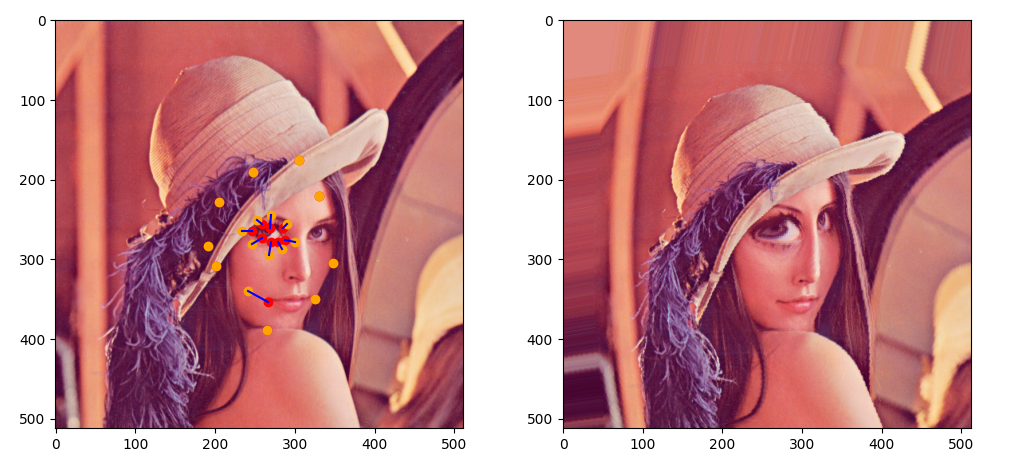
\includegraphics[width=0.6\textwidth]{./Figure/HW2-example.png}
        \caption{Image warping example}
        \label{fig:image-warping}
\end{figure}

\newpage

\begin{solution} \textbf{High-Dimensional Linear Regression for Image Warping}
\begin{enumerate}
	\item
	Define
	\[
	\mathbf{X}
	=
	[\mathbf{x}_1, \mathbf{x}_2, \dots, \mathbf{x}_N] \in \mathbb{R}^{n \times N},
	\qquad
	\mathbf{Y} = [\mathbf{y}_1, \mathbf{y}_2, \dots, \mathbf{y}_N] \in \mathbb{R}^{m \times N}
	\]
	\[
	\mathbf{\Phi} \in \mathbb{R}^{N \times N}, (\mathbf{\Phi})_{ij} = \phi_j(\mathbf{x}_i)
	\qquad
	\mathbf{1}_N = (1,1,\dots,1)^T \in \mathbb{R}^N
	\]
	\begin{align*}
	\Longrightarrow
	l
	&=
	\sum_{i = 1}^N\left\Vert \hat{\phi}(\mathbf{x}_i) - \mathbf{y}_i \right\Vert _2^2 + \lambda_1\Vert \mathbf{A} - \mathbf{I}\Vert_f^2 + \lambda_2 \Vert\mathbf{b} \Vert _2^2 + \lambda_3\Vert \mathbf{W}\Vert_f^2\\
	&=
	\left\Vert \mathbf{A}\mathbf{X} + \mathbf{b}\mathbf{1}_N^\top + \mathbf{W} \mathbf{\Phi} - \mathbf{Y} \right\Vert _f^2
	+
	\lambda_1\Vert \mathbf{A} - \mathbf{I}\Vert_f^2
	+
	\lambda_2 \Vert\mathbf{b} \Vert _2^2
	+
	\lambda_3\Vert \mathbf{W}\Vert_f^2
	\end{align*}
	\begin{equation}
	\nonumber
	\Longrightarrow
	\left\{
	\begin{aligned}
	&\partial_\mathbf{W} l
	=
	2\left(\mathbf{A}\mathbf{X} + \mathbf{b}\mathbf{1}_N^\top + \mathbf{W} \mathbf{\Phi} - \mathbf{Y}\right) \mathbf{\Phi}^\top + 2\lambda_3 \mathbf{W}
	=
	0\\
	&\partial_\mathbf{A} l
	=
	2\left(\mathbf{A}\mathbf{X} + \mathbf{b}\mathbf{1}_N^\top + \mathbf{W} \mathbf{\Phi} - \mathbf{Y}\right) \mathbf{X}^\top + 2\lambda_1 (\mathbf{A} - \mathbf{I})
	=
	0\\
	&\partial_\mathbf{b} l
	=
	2\left(\mathbf{A}\mathbf{X} + \mathbf{b}\mathbf{1}_N^\top + \mathbf{W} \mathbf{\Phi} - \mathbf{Y}\right) \mathbf{1}_N + 2\lambda_2 \mathbf{b}
	=
	0
	\end{aligned}
	\right.
	\end{equation}
	\begin{equation}
	\nonumber
	\Longrightarrow
	\left\{
	\begin{aligned}
	&\mathbf{W}^*
	=
	\left(\mathbf{Y} - \mathbf{A}^*\mathbf{X} - \mathbf{b}^*\mathbf{1}_N^\top\right) \mathbf{\Phi}^\top
	\left(\mathbf{\Phi} \mathbf{\Phi}^\top + \lambda_3 \mathbf{I}\right)^{-1}\\
	&\mathbf{A}^*
	=
	\left(\left(\mathbf{Y} - \mathbf{b}^* \mathbf{1}_N^\top - \mathbf{W}^* \mathbf{\Phi}\right) \mathbf{X}^\top + \lambda_1 \mathbf{I}\right) \left(\mathbf{X} \mathbf{X}^\top + \lambda_1 \mathbf{I}\right)^{-1}\\
	&\mathbf{b}^*
	=
	\left(N + \lambda_2\right)^{-1} \left(\mathbf{Y} - \mathbf{A}^* \mathbf{X} - \mathbf{W}^* \mathbf{\Phi}\right) \mathbf{1}_N
	\end{aligned}
	\right.
	\end{equation}
	\item 	
\end{enumerate}
\end{solution}
    
\newpage
\begin{exercise}[Bias-Variance Trade-off (Programming Exercise) ]\label{BiasVariance}
    We provide you with $L=100$ data sets, each having $N=25$ points:
    $$
    \mathcal{D}^{(l)}=\{ (x_n,y_n^{(l)})\}_{n=1}^N,\quad l=1,2,\cdots ,L,
    $$
    where $x_n$ are uniformly taken from $[-1,1]$, and all points $(x_n, y_n^{(l)})$ are independently from the sinusoidal curve $h(x)=\sin (\pi x)$ with an additional disturbance.
    \begin{enumerate}
        \item For each data set $\mathcal{D}^{(l)}$, consider fitting a model with $24$ Gaussian basis functions
        \begin{align*}
            \phi_j(x)= e^{-(x-\mu_j)^2},\quad \mu_j = 0.2 \cdot (j-12.5),\quad j = 1,\cdots 24
        \end{align*}
        by minimizing the regularized error function
        \begin{align*}
            L^{(l)}(\mathbf{w}) = \frac{1}{2}\sum_{n=1}^N (y^{(l)}_n - \mathbf{w}^\top \bm{\phi}(x_n))^2 + \frac{\lambda}{2}\mathbf{w}^\top\mathbf{w},
        \end{align*}
        where $\mathbf{w}\in\mathbb{R}^{25}$ is the parameter, $\bm{\phi}(x)=(1, \phi_1(x),\cdots,\phi_{24}(x))^\top$ and $\lambda$ is the regular coefficient. What's the closed form of the parameter estimator $\hat{\mathbf{w}}^{(l)}$ for the data set $\mathcal{D}^{(l)}$?

        \item For $\log_{10}\lambda = -10, -5,-1,1$, plot the prediction functions $y^{(l)}(x)=f_{\mathcal{D}^{(l)}}(x)$ on $[-1,1]$ respectively. For clarity, show only the first $25$ fits in the figure for each $\lambda$.

        \item For $\log_{10}\lambda\in [-3,1]$, calculate the followings:
        \begin{align*}
            \bar{y}(x)& =\mathbb{E}_{\mathcal{D}}[f_{\mathcal{D}}(x)]=\frac{1}{L}\sum_{l=1}^L y^{(l)}(x) \\
            (\mbox{bias})^2& =\mathbb{E}_X[(\mathbb{E}_{\mathcal{D}}[f_{\mathcal{D}}(X)]-h(X))^2]=\frac{1}{N}\sum_{n=1}^N (\bar{y}(x_n)-h(x_n))^2\\
            \mbox{variance} &= \mathbb{E}_X[\mathbb{E}_{\mathcal{D}}[(f_{\mathcal{D}}(\mathbf{x})-\mathbb{E}_{\mathcal{D}}[f_{\mathcal{D}}(\mathbf{x})])^2]] = \frac{1}{N}\sum_{n=1}^N\frac{1}{L}\sum_{l=1}^L (y^{(l)}(x_n)-\bar{y}(x_n))^2
        \end{align*}
        Plot the three quantities, $(\mbox{bias})^2, \mbox{variance}$ and $(\mbox{bias})^2 + \mbox{variance}$ in one figure, as the functions of $\log_{10}\lambda$.
        (\textbf{Hint:} see \cite{Bishop2006} for an example.)
    \end{enumerate}

\end{exercise}



% \newpage
% \begin{exercise}[(Optional) Positive Semi-definite Matrices and the Polyhedron]
% Please show that Sn+\mathbb{S}_+^n is not a polyhedron.

% \end{exercise}

% \newpage
% \begin{exercise}[Convex Sets]
%     Let C⊂RnC \subset \mathbb{R}^n be a nonempty convex set. Please show the following statements.
%     \begin{enumerate}
%       \item Please find the interior and relative interior of the following convex sets (you don't need to prove them).
%       \begin{enumerate}
%           \item {x∈R3:x21+x22<1,x3=0}⊂R3\{\mathbf{x}\in\mathbb{R}^3: x_1^2+x_2^2<1,x_3=0\}\subset\mathbb{R}^3.
%           \item {A∈Sn++:Tr(A)=1}⊂Rn×n\{\mathbf{A}\in S_{++}^n: \text{Tr}(\mathbf{A})=1\}\subset \mathbb{R}^{n\times n}.
%           \item {A∈Sn++:Tr(A)=1}⊂Sn\{\mathbf{A}\in S_{++}^n: \text{Tr}(\mathbf{A})=1\}\subset S^ n.
%           \item (Optional) {A∈Sn++:Tr(A)≤1}⊂Rn×n\{\mathbf{A}\in S_{++}^n: \text{Tr}(\mathbf{A})\le1\}\subset \mathbb{R}^{n\times n}.
%           % \item \conv({x,x2,x3})⊂C[0,1]\conv (\{x, x^2, x^3\})\subset C[0,1] with L∞L^\infty norm, i.e., ‖\|f\|_\infty = \max_{x\in [0,1]}|f(x)| for any f\in C[0,1]f\in C[0,1].
%       \end{enumerate}
%       \item  Some operations that preserve convexity.
%       \begin{enumerate}
%         \item
%         Both \clC\cl C  and \intpC\intp C  are convex.
%         \item
%         The set \relintC\relint{C} is convex.
%         \item
%         The intersection ⋂i∈ICi\bigcap_{i \in I}C_i of any collection {Ci:i∈I}\{ C_i:i\in \mathcal{I} \} of convex sets is convex.

%         \item
%         The set {y∈Rm:y=Ax+a,x∈C}\{ \mathbf{y}\in\mathbb{R}^m:\mathbf{y}=\mathbf{Ax}+\mathbf{a},\mathbf{x}\in C \} is convex, where A∈Rm×n\mathbf{A} \in \mathbb{R}^{m \times n} and a∈Rm\mathbf{a} \in \mathbb{R}^m.
%         \item
%         The set {y∈Rm:x=By+b,x∈C}\{ \mathbf{y}\in\mathbb{R}^m:\mathbf{x}=\mathbf{By}+\mathbf{b},\mathbf{x}\in C \} is convex, where B∈Rn×m\mathbf{B} \in \mathbb{R}^{n \times m} and b∈Rn\mathbf{b} \in \mathbb{R}^n.
%     \end{enumerate}

%     \end{enumerate}

% \end{exercise}
% \begin{solution}

% \end{solution}

% \footnotetext{You will attain \textbf{one extra point} of bonus in your \textbf{final rating} if you work out this problem.}
%%%%%%%%%%%%%%%%%%%%%%%%%%%%%%%%%%%%%%%%%%%%%%%%%%%%%%%%%%%%%%%%
	
	\newpage
    \bibliography{refs}
    \bibliographystyle{abbrv}
	

\end{document}
